%
% PROJECT: <ETD> Electronic Thesis
%   TITLE: Looks Good to Me (LGTM): Authentication for Augmented Reality
%  AUTHOR: Ethan Gaebel
% SAVE AS: thesis-draft.tex
% 

\documentclass[12pt]{report}
%\documentclass[12pt,dvips]{report} -- ORIGINAL


\usepackage{graphicx}

\setlength{\textwidth}{6.5in}
\setlength{\textheight}{8.5in}
\setlength{\evensidemargin}{0in}
\setlength{\oddsidemargin}{0in}
\setlength{\topmargin}{0in}

\setlength{\parindent}{0pt}
\setlength{\parskip}{0.1in}

% Uncomment for double-spaced document.
% \renewcommand{\baselinestretch}{2}

% \usepackage{epsf}

\begin{document}

\thispagestyle{empty}
\pagenumbering{roman}
\begin{center}

% TITLE
{\Large 
Looks Good to Me (LGTM): 
Authentication for Augmented Reality
}

\vfill

Ethan D. Gaebel

\vfill

Thesis submitted to the Faculty of the \\
Virginia Polytechnic Institute and State University \\
in partial fulfillment of the requirements for the degree of

\vfill

Master of Science \\
in \\
Computer Science and Applications

\vfill

Wenjing Lou, Committee Chair \\
Ing-Ray Chen \\
Guoqiang Yu 

\vfill

May 15, 2016 \\
Falls Church, Virginia

\vfill

Keywords: 
\\
Copyright 2016, Ethan D. Gaebel

\end{center}

\pagebreak

\thispagestyle{empty}
\begin{center}

{\large Looks Good to Me (LGTM): 
Authentication for Augmented Reality}

\vfill

Ethan D. Gaebel

\vfill

(ABSTRACT)



\vfill

\end{center}

Security-based abstract and stuff!!!

\vfill

% GRANT INFORMATION
This work was supported in part by the National Science Foundation under Grants 
CNS-1443889, CNS-1405747, CNS-1446478, and CNS-1343222.

\pagebreak

% Dedication and Acknowledgments are both optional
% \chapter*{Dedication}
% \chapter*{Acknowledgments}

\tableofcontents
\pagebreak

\listoffigures
\pagebreak

\listoftables
\pagebreak

\pagenumbering{arabic}
\pagestyle{myheadings}

%%%%%%%%%%%%%%%%%
\chapter{Introduction}
\markright{Ethan D. Gaebel \hfill Chapter 1. Introduction \hfill}
% Augmented Reality
% ---- Convince readers it is the future
% ---- Discuss options for AR: headsets, hardware included, etc
% ---- Augmented reality NEEDS a device pairing mechanism
% ---- Why pair point-to-point?
% -------- More efficient network resource usage
% --------- Problem is inherently local
% -------- Not reliant on infrastructure, more robust to patchy areas
% ------------ Cheaper if we consider the non-WiFi usage 
% ---------------- WAY cheaper if you further consider the content size!
% ---- Preserves privacy
% Augmented reality needs device pairing
% ---- Sharing holograms, etc
% Device Pairing
% ---- Difficulty of bootstrapping authentication
% ---- Man-in-the-middle (MOVE)
% ---- Evil twin (MOVE)
% ---- The Resurrecting Duckling (MOVE)
% ---- Long history, briefly summarize to illustrate the breadth of techniques investigated
% ---- Difficulty of pairing over wireless channel 
% ---- Usability's importance to security in practice
% ---- Pin currently dominant method
% ---- Mention centralized device pairing methods.... (this is kind of out of the purview of device pairing; a user account can be used to bootstrap?)
% Augmented reality can have BETTER device pairing
% ---- Improved hardware and user interface provides avenue for BETTER device pairing (better = more usable --> more secure)
% -------- Must be more usable than a pin
% High level description of LGTM from the user perspective (high level even for the user view)
% ---- Press button, look at other person, etc
% ---- Compare EM waves & sound waves for localization & information carrying purposes
% ---- How does this look formally? (transition)
\section{Augmented Reality}
% What is it?
% ---- Digital ON reality
% How's it done?
% ---- Briefly mention alternatives, but get specific about HMDs
% ---- Display
% ---- Interaction
% ---- Standard hardware

% Why should we do it?
% ---- Richer content
% ---- More interactive
% -------- While retaining existing interfaces too (purely additive)
% Current industry state
% ---- Opportunity to influence development

% Segway about richer, in-person content 

\section{Face-to-Face Sharing}
% Relation to AR (why?)
% History (of sharing)
% ---- Internet, etc
% -------- Reasons behind this
% Why face-to-face sharing?
% ---- YouTube video sharing comment
% ---- Sharing, user interaction
% ---- Somehow quote the Meta CEO about not being taken out of the real world
% How do we do face-to-face-sharing
% ---- P2p wireless
% ---- Real examples (WiFi direct, Bluetooth)
% ---- Real examples in-use (Firechat, etc)
% ---- Why NOT traditional means
% -------- Network congestion
% -------- Latency
% -------- Lack of service (airplanes, rural areas, etc)
% Problems to conquer? (act as segway)
% ---- Authentication
% ---- Mention (not in-depth) security issues with spamming vision
% -------- I can do a LOT of expansion here
% -------- Make this VERY, VERY grabby


\section{Face-to-Face Authentication}
\subsection{Device Pairing}
% History (device pairing)
% ---- Diverse hardware & creative solutions
% ---- OOB solutions (segway)

\subsection{Human Component}
% Human component (in pairing generally)
% Verifier
% Facilitator of OOB channel (pin, etc)
% Segway into usability (should be a pretty natural/easy segway)


\section{Usability}
% What is it? (ISO definition)
% Why is it important (generally) ?
% ---- User confusion
% ---- Technology should make things easier!
% Why is it important (security) ?
% ---- Explanation
% ---- Evidence (studies)
% Relation to AR (Generally)
% ---- More immersion --> more "real" interface
% Relation to AR (for Security (expand from generally))
% ---- Connect prior points to security
% ---- Connect to how humans have always done security
% -------- "Security is becoming more complex, but more familiar. Humans have always had to secure things from each other...we're raising computer security back up to human security, making it harder to analyze, but easier to deal with."

% Segway to LGTM

%%%%%%%%%%%%%%%%%
\chapter{LGTM Protocol}
\section{Security Opportunities with AR}
% Security opportunities
% ---- Hardware
% ---- User Setting
% Intuition/Analogy (THE analogy)
% Pull reader in with question (THE question)

% Transition to formality

\section{System Model}
% System Model
% ---- Protocol hardware requirements
% -------- Users have augmented reality head-mounted displays equipped with:
%               wireless communications, support for point-to-point 
%               communications, high resolution cameras, relatively good 
%               computational abilities, and translucent screens very close to 
%               the eye such that only the user can reasonably see them which 
%               are capable of rendering 2D and 3D objects on top of the 
%               physical world which the user is already seeing.
% ---- Users are present, in-person/face to face, and would like to establish 
%           communication to share some kind of content between their devices 
%           which may include: a shared app experience, watching a video, 
%           listening to the same music, shared holograms, basic messaging
% ---- Users of LGTM have no prior security context with regard to their 
%           devices; the users may be friends, acquaintances or strangers.
% ---- Each user possesses, in the memory of their augmented reality headsets, 
%           facial recognition models for themselves.
% -------- These are easily trained via mirror.
% ---- No assumptions regarding access to the Internet are made.

\section{Threat Model}
% Threat Model
% ---- Wireless attacker model

\section{Security Objectives}
% (Security) Objectives
% ---- Authenticate the wireless signal of one user so that secure 
%           communication can be done between two individuals
% -------- Bootstrapping authentication
% ---- Select a user-wireless signal pair to communicate with
% -------- Selection problem
% ---- Privacy Objectives (sub-section under security objectives...)
% -------- No need for centralized power knowing communication/content patterns
% -------- Intermediary parties facilitating communication is 0
% ------------ The potential for remote eavesdropping, censorship, tracking, 
%                   etc, is non-existent

\section{Protocol}
% Protocol, high level (high-level, as in the protocol diagram)

% Protocol Figure
\begin{figure}
\center
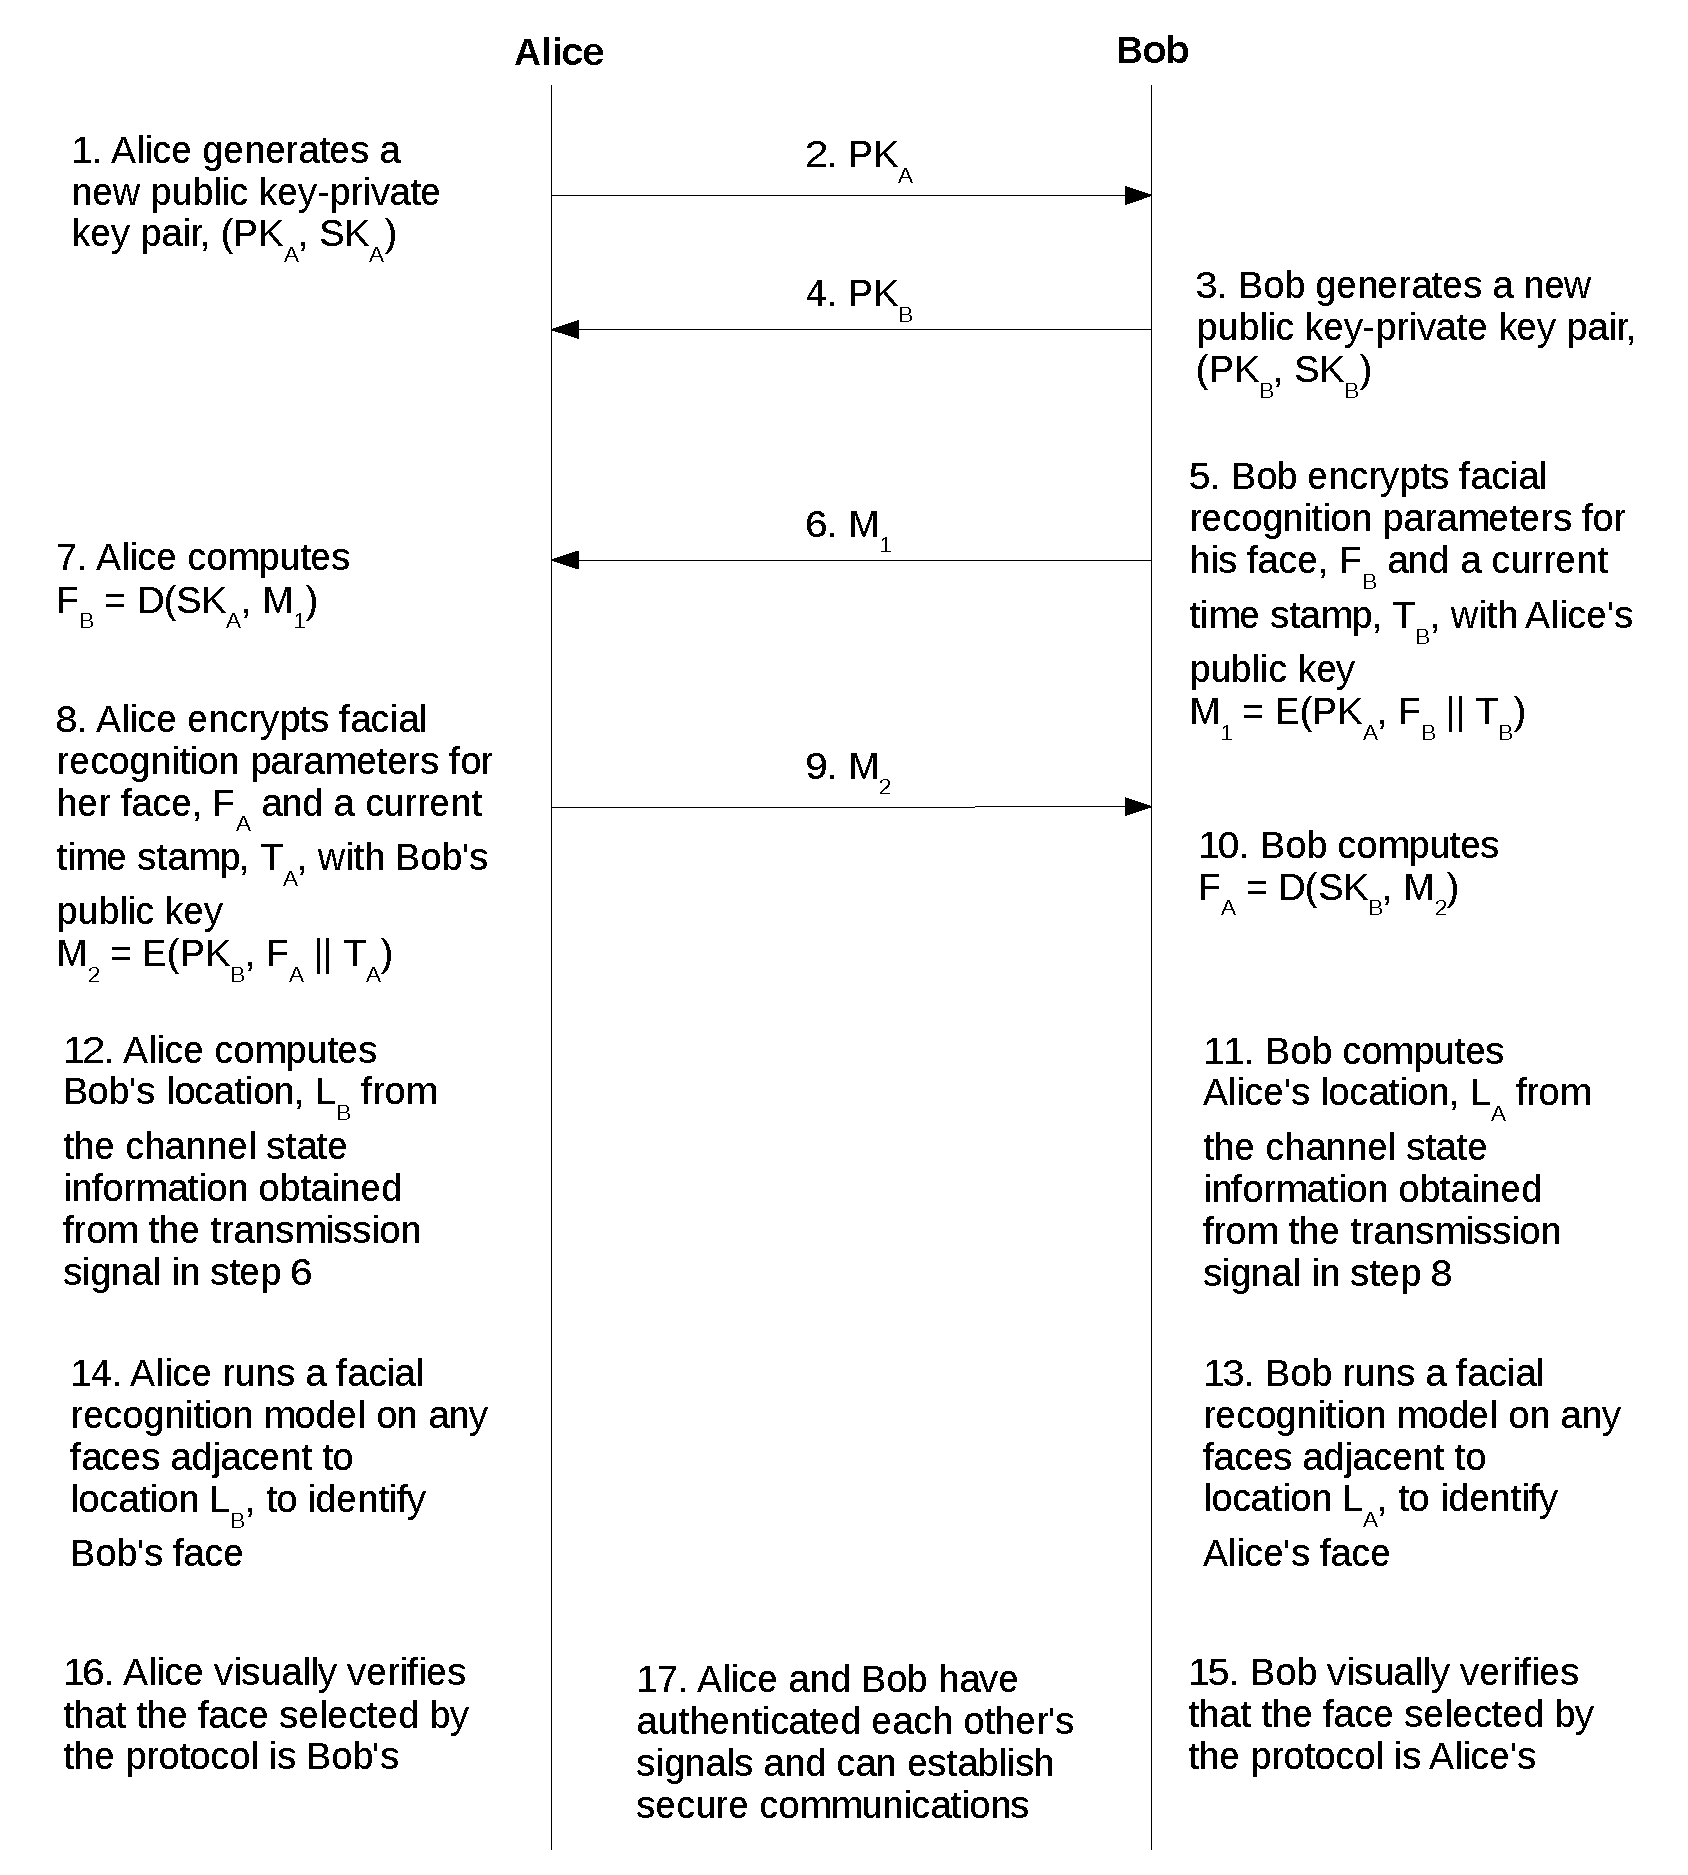
\includegraphics[scale=0.6]{../figures/looks-good-to-me-protocol-diagram--no-legend.pdf}
\caption{Looks good to me protocol diagram...}
\label{protocol-diagram}
\end{figure}

% Protocol, specific (Alice receives $n$ packets, etc...)

\section{Analysis}
% Protocol Analysis
% ---- Describe each step of the protocol (protocol specific above?)


\subsection{Protocol Techniques (Workshop this name..it isn't GREAT)}

\subsubsection{Public-Key Cryptography}
% Role: Bootstrapping symmetric key cryptography, prevents eavesdroppers
%       from learning parameters needed to derive symmetric key
% Details: Algorithm examples (Diffie-Hellman, RSA, etc)
% Considerations: # bits, key policy, specific technique used to establish key

\subsubsection{Symmetric-Key Cryptography}
% Role: Provides confidentiality
% Details: Algorithm example (AES), key establishment parameters (nonces)
% Considerations: # bits, mode of operation (CBC, GCM, etc)

\subsubsection{Message Authentication}
% Role: Provides message stream authentication, which acts as a secure session key
% Details: Algorithm examples (SHA2, SHA3)
% Considerations: # bits, what is input (everything prior + 'this' (unencrypted))

\subsubsection{Localization}
% Role: Provides user authentication, by revealing signal origin (then match up with device/user)
% Details: Accuracy considerations & effects on security
% Considerations: Attack space, performance, increasing accuracy, ideas regarding security uses (other than LGTM)

\subsubsection{Facial Recognition}
% Role: Eases user-selection problem, makes authentication easier by removing users not in the valid area automatically
% Details: Accuracy, Performance (time)
% Considerations: Facial detection + facial recognition (two steps needed), increasing accuracy, facial recognition already used for security purposes, include conversation about how it provides security against unplanned attacks (it's hard to get a facial recognition model trained on someone you see only briefly)

\subsubsection{Human Verification}
% Role: Spoof detection, solving user-selection
% Details: Human facial recognition abilities (VERY, VERY GOOD)


\subsection{Security Against Attacks} % PENDING STORYBOARDING!!!
% Security
% ---- Wireless attacks
% -------- Jamming 
% ------------ Works on any wireless pairing technique
% -------- DOS, spam the user(s) with auth requests 
% ------------ Works on any wireless pairing technique
% -------- Man-in-the-middle
% ------------ Works on any wireless pairing technique
% ------------ Wait...the feasibility depends on the quality of the wireless 
%                   localization. In a perfect implementation, this won't work.
% ---- Attacker ability is based on the quality of the facial recognition 
%           & wireless localization (correctness)
% -------- "Attack space" for wireless localization
% ---- Why not a pin?


\subsection{Usability}
% Usability
% ---- Why not a pin?
% -------- Greater range; you can see farther than you can hear
% -------- Will not work in loud environments
% -------- Will not work for the deaf (LGTM won't work for the blind, but 
%                   neither will AR in general, and neither will a pin)
% -------- Depending on implementation, may be less secure, overhearing 
%                   pin can be a security leak

\subsubsection{LGTM Puts Usability First (WORKSHOP THIS TITLE, IT SUCKS)}
% Usability is good for users (for products, etc)
% Usability impacts security
% ---- Examples: Phishing, case studies, trojans, click-bait, etc

% Facial recognition improves usability
% ---- Bring up alternative localization sphere
% ---- Humans have a fantastic ability to recognize faces (bringing up AGAIN)
% ---- In standard case (non-malicious) selections can be auto-eliminated if faces & localization don't line up, leading to fewer user choices, which is always more usable
% -------- Link back to usability leading to more security

% Wireless p2p improves usability
% ---- ALWAYS available
% -------- No Internet, no problem
% -------- Bring up relatable analogies (on the plane, basic lack of service, geographically lacking quality service (rural areas, Kansas))
% ---- Centralized infrastructure requires secondary authentication
% -------- "Yo dawg, you need to authenticate so you can authenticate"
% -------- This is LESS usable, more steps, more room for mistakes, more room for bugs (security tie in again?)

% LGTM Approaches MAX usability
% ---- It's how we authenticate human speakers!
% ---- Only two user actions, begin, and confirm (how can you reduce from that?)

\subsection{Privacy} % (This will not be a particularly long sub-section...)
% People ARE interested in privacy
% ---- Cite study about the % of people who have taken steps to improve their privacy online
% P2p wireless forces data collection to occur VERY close up
% ---- P2p forces attackers to be nearby
% ---- Long term collection requires straight-up stalking (infeasible)
% Central Authority drawbacks
% ---- Central authorities can EASILY monitor:
% -------- Who you talk to
% -------- What you send
% -------- When you send
% ---- Central authorities are indeed INCENTIVIZED
% -------- Data mining, etc
% The best way to protect against centralized data collection is to not use a centralized method of sharing
% ---- This has been inefficient in the past (sharing with people not nearby)
% ---- This is a better idea now (sharing will occur up close, enhancing real life)
% Short conclusion
% ---- LGTM improves privacy in comparison to centralized communications
% -------- Only possible due to AR specific use-cases


\subsection{Potential Alterations}  % Should this section be here?
% Expanding to the group case
% One way sharing: (I.E. Alice receives content from Bob, but not vice-versa)

%%%%%%%%%%%%%%%%%
\chapter{Implementation}
% General setup
% ---- AR headsets unavailable (expensive, not powerful enough yet, not 
%           flexible enough yet)
% ---- Necessary components from AR headsets for experimental purposes (
%           Wireless, video camera, display)
% Wireless Localization Discussion
% ---- Discuss past localization techniques, BRIEFLY
% ---- Discuss lack of focus on point-to-point localization
% ---- Discuss new protocols that enable point-to-point localization in 
%           commodity hardware
% Facial Recognition Discussion
% ---- Very brief discussion of techniques, the area is well studied and my 
%           techniques are not new
% Specific Wireless localization and facial recognition methods
% ---- SpotFi
% ---- OpenCV
% -------- Fisherfaces, LBPH, Haarcascade, etc
% Specific localization & facial recognition components
% ---- Intel 5300 firmware etc
% ---- Laptops with web cams and three antennas each
% System and Validation
% ---- Glue code, system structuring, specifics of protocol implementation
% ---- Explain each implementation decision, why and how, discuss alternatives
% ---- This section should mainly discuss why certain things were NOT done, 
%           and why things ARE done 
% -------- belongs under "General Setup"

\section{Test Bed} % (high level explanation)
% Why LGTM cannot be implemented on real AR systems
% ---- Availability
% ---- Lack of open firmware for wireless localization
% My solution
% ---- Necessary conditions for LGTM that AR satisfies:
% -------- High-definition video camera
% -------- Wireless p2p communications capabilities
% -------- Wireless localization capabilities
% -------- Proximity of face to wireless communications
% -------- Screen
% -------- Computational abilities
% ---- Web cam
% ---- Wireless card with open firmware to grab CSI
% ---- array of 3 antennas
% ---- Pictures of faces on top of the arrays
% ---- Laptop


\section{Technologies}

\subsection{Encryption}
\subsubsection{Public-Key}
% Elliptic curve diffie-hellman, # bits

\subsubsection{Symmetric-Key}
% AES-256
% CBC OR GCM mode? 
% Initialization vector

\subsubsection{Message Authentication Codes (MACs)}
% SHA-512, SHA3, etc


\subsection{Localization}
% Brief overview of approaches
% ---- AoA, RSSI, fingerprinting, etc
% AoA based localization
% ---- MUSIC
% 802.11n properties (OFDM etc)
% SpotFi
% SpotFi Tweaks

\subsection{Facial Detection}
% Haarcascades

\subsection{Facial Recognition}
% Eigenfaces (brief + why not used)
% Fisherfaces (brief + why not used)
% Local Binary Pattern Histograms

\section{Hardware}
% Laptops + specs + OS
% Wireless cards
% ---- Explain why the Intel 5300 was chosen
% -------- Firmware
% -------- Extra software
% -------- More elaboration under software section
% Antennas
% ---- Spacing
% ---- Positioning on laptops 
% ---- Location relative to face print outs
% Web cams
% ---- Manufacturer information + model
% ---- Field of view
% ---- Resolution
% ---- Frame rate

\section{Software}
% Extensive section right here
% OS
% ---- Why?
% -------- Firmware
% -------- Linux tools (bash, etc)
% -------- Unparalleled support

% Component-by-component break-down
% ---- Firmware loading/unloading
% ---- Wireless parameter settings
% -------- ip command
% -------- iw command
% -------- Error/timing tolerance fixes

% Packet Sending/Receiving
% ---- Halperin
% ---- LORCON
% ---- Filesystem
% ---- C

% Packet CSI collection
% ---- Halperin
% ---- MATLAB
% ---- C

% Packet Decoding
% ---- Halperin
% ---- MATLAB

% SpotFi
% ---- MATLAB
% ---- Speed ups (par for)
% ---- Algorithm 1
% ---- Clusteirng algorithm
% ---- MUSIC
% ---- Parameter learning (SVM + data)

% Facial Detection & Recognition
% ---- OpenCV
% ---- C++
% ---- AoA and face match up
% ---- User confirmation & input
% ---- Live video
% ---- LBPH and Haarcascade usage and details
% -------- Training & Testing

% Cryptography 
% ---- Crypto++
% ---- C++
% ---- Linux file system

% Bash script for glue
% ---- File system usage
% ---- Linux tool usage
% ---- User input
% ---- Modularity
% ---- Ideal for debuggin (file-by-file)

% Full System Walk-through
% ---- Data flow diagrams
% ---- Control flow diagrams
% ---- Walk-through (high level) of program execution with references to the components

% Data Analysis Scripts (Maybe include, maybe don't....)
% ---- Python
% ---- Parsing output
% ---- Computing statistics
% ---- Allows for high output volume (lots of testing)
%%%%%%%%%%%%%%%%%
\chapter{Experiments}
% Experiments (Very formal)
% ---- Security
% ---- Performance
% ---- SpotFi Accuracy
% -------- Effective "attack space"
% ---- Facial recognition accuracy
% Results (for each above)
% Discussion (for each above)

%%%%%%%%%%%%%%%%%
\chapter{Conclusion}
% List of points to hit on:
% ---- Oldness and difficulty of device pairing
% ---- Usability's impact on security
% ---- Ease of use of LGTM
% ---- Point-to-point communication providing privacy
% ---- Something optimistic and feel-good sounding about the future

%%%%%%%%%%%%%%%%%
%
% Include an EPS figure with this command:
%   \epsffile{filename.eps}
%

%%%%%%%%%%%%%%%%
%
% Do tables like this:

% \begin{table}
% \caption{The Graduate School wants captions above the tables.}
% \begin{center}
%  \begin{tabular}{ccc}
%  x & 1 & 2 \\ \hline
%  1 & 1 & 2 \\
%  2 & 2 & 4 \\ \hline
%  \end{tabular}
% \end{center}
% \end{table}

%%%%%%%%%%%%%%%%%%%%%%%%%%%%%%%%

% If you are using BibTeX, uncomment the following:
% \thebibliography
%
% Otherwise, uncomment the following:
% \chapter*{Bibliography}

% \appendix

% In LaTeX, each appendix is a "chapter"
% \chapter{Program Source}


\end{document}